\documentclass[10pt,a4paper]{article}
\usepackage{listings}
\usepackage[utf8]{inputenc}
\usepackage{color}
\usepackage[francais]{babel}
\usepackage[T1]{fontenc}
\usepackage{graphicx}
\usepackage[export]{adjustbox}
\bibliographystyle{ieeetr}
\author{Ali CHERIFI}
\title{Rapport de stage de licence\\Résumé vidéo et vidéo 3D anaglyphe et side-by-side}
\begin{document}
\maketitle
\newpage
\tableofcontents
\newpage
\section{Introduction}
Le relief de la vision humaine provient de la différence de perception entre les deux yeux. La stéréoscopie rassemble toutes les différentes méthodes permettant de reconstruire cet effet à partir d'objets 2D
observés soit à travers un instrument d'optique ou alors à partir de deux photographies prises avec un décalage.
La stéréoscopie est un domaine qui a interessé l'homme depuis longtemps. En effet, ce principe a été imaginé par Charles Wheatstone\cite{stereoscopie} (physicien et inventeur anglais) en 1832.
Le premier appareil créant l'effet stéréoscopique a vu le jour en 1843 par David Brewster (physicien et inventeur écossais). Cet appareil ne servait alors qu'à observer deux dessins.
Cet appareil monta en popularité avec l'apparition des travaux sur la photographie. Il était constitué de deux prismes comportant chacun des faces convexes. Cela permettait à chaque oculaire de
produire à la fois l'effet d'un prisme et d'une lentille. L'impression de relief était donc observable sur deux photographies dont le centre de la deuxième est décalé de quelques centimètres.

\begin{figure}[!h]
\center
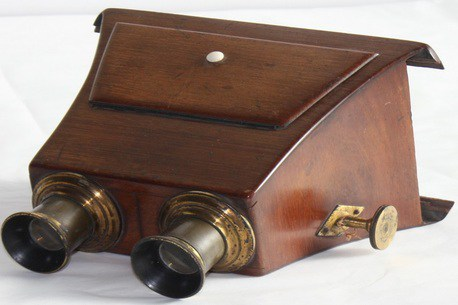
\includegraphics[scale = 0.5]{brewer.jpg}
\caption{Stéréoscope de Brewer\cite{brewster}.}
\end{figure}

Un procédé voisin mais néanmoins différent est celui de l'anaglyphe. Ce procédé sera décrit plus en détail dans la section\ref{anasbs}.
Actuellement les dispositifs les plus populaires s'inspirent du stéréoscope de Brewer pour reconstruire le relief comme le fait l'Oculus Rift ou l'HTC Vive. La technologie side-by-side est utilisée ici et sera vu en détail dans la section \ref{anasbs}.

Ces deux procédés ont très vite été adaptés aux vidéos afin de rendre les films plus vivants et réels et ainsi augmenter l'immersion.
A l'heure actuelle tous ces procédés utilisent deux photographies ou vidéos prisent avec un point de vue différents  Le rendu du relief est alors très convaincant car très proche de la réalité.
Cependant, se procurer deux caméras ou appareils photos est très onéreux et n'est pas à la portée de tout le monde. 

Le but ici sera donc de réfléchir et de trouver un moyen de produire cet effet de stéréoscopie à partir d'une seule source vidéo ou d'une seule photographie tout en obtenant un relief le plus convaincant possible. Le résultat ne sera cependant jamais le même qu'avec deux images,
la perspective étant fixe à partir d'une seule source. Lors d'une prise avec deux appareils, certains éléments sortent du cadre de la photo tandis que d'autres y entrent. La quantité d'informations présente sur une image est fixe. La translation qui se fera pour produire le décalage entre les deux yeux constituera alors une perte d'informations sans aucun gain.

Le but ici est donc d'automatiser le processus de création d'une vidéo stéréoscopique anaglyphe et side-by-side à partir d'une seule source vidéo tout ceci en JAVA.

\section{Laboratoire d'accueil}

Mon stage est effectué au sein du LaBRI, le Laboratoire Bordelais de Recherche en Informatique. Le LaBRI est associé au CNRS, à l'Université de Bordeaux ainsi qu'à l'INP (Institut Polytechnique de Bordeaux)\cite{labri}.
Le LaBRI compte environ 300 personnes dont 113 enseignants et chercheurs de l'Université de Bordeaux et de L'INP et 37 chercheurs répartis entre L'INRIA (Institut National de Recherche en Informatique et en Automatique) et le CNRS. Le LaBRI compte également 140 doctorants, post-doctorants et ingénieurs contractuels.
Six équipes existent au sein du LaBRI axant leur recherche sur différents domaines. Les équipes sont les suivantes :\\

\begin{itemize}
\item Combinatoire et Algorithmie
\item Méthodes Formelles
\item Modèles et Algorithmes pour la Bioinformatique et la Visualisation d'informations
\item Programmation, Réseaux et Systèmes
\item Supports et Algorithmes pour les Applications Numériques Hautes performances.
\item Image et Son\\
\end{itemize}

Mon stage s'effectuera au sein de l'équipe Image et Son.

\section{Etat de l'art et matériel existant}


\subsection{Résumé vidéo}

Le résumé vidéo peut aussi être appelé "Movie Barcode". Il permet de faire ressortir la couleur générale d'un film ou d'une vidéo(voir figure 
En récupérant la bande du milieu de chaque image et en concaténant tout cela pour
tout le film, on obtient une image très similaire à un code barre représentant l'ambiance générale de la vidéo.

Il existe un logiciel disponible réalisant ce traitement nommé "Movie Barcode Generator". Le logiciel est écrit en C\# et ses sources sont disponibles à tous\cite{barcode}. L'auteur du logiciel accepte la vente des résultats produit par son logiciel (voir figure \ref{moviebarcodegenerator}).
\begin{figure}[h]
\center
\includegraphics[scale = 0.3]{barcode.jpg}
\caption{Image générée par Movie Barcode Generator pour le film \textit{The Revenant}.}
\label{moviebarcodegenerator}
\end{figure}


\newpage
\subsection{Anaglyphe et side-by-side}
\label{anasbs}
Actuellement, le vidéo 3D par anaglyphe propose deux méthodes majeures, un algorithme simple et la méthode de Dubois.
Le premier algorithme consiste à séparer et à extraire les canaux RGB d'une image 2D et d'en faire une image 3D. Le principe réside dans le filtrage des couleurs par l'œil devant lequel se trouve un filtre.
Chaque œil ayant un filtre différent, il ne perçoit que les couleurs que le filtre laisse passer. Actuellement, le filtre le plus répandu est le filtre rouge/cyan.
Il suffit donc dans le cas de cet algorithme, d'extraire le canal rouge de l'image et d'en générer un nouvelle. Ensuite il faut à partir de l'image source créer une nouvelle image à partir du mélange des canaux bleu et vert.
On obtient ainsi deux images, une cyan et l'autre rouge. Il faut ensuite les superposer en leur appliquant un décalage(voir figure \ref{anaglyphe}).\newline

\begin{figure}[!h]
\center
\includegraphics[scale = 0.5]{anaglyphe.jpg}
\caption{Image anaglyphée.}
\label{anaglyphe}
\end{figure}

Éric Dubois est ingénieur et chercheur à l'Université d'Ottawa au Canada\cite{duboisbio}. Ses travaux sur la stéréoscopie commencent lors d'un projet en collaboration avec IMAX\footnote{Entreprise ayant mis au point le format IMAX, dix fois plus large que les tailles d'écrans de cinéma classique.}. Éric Dubois propose de modifier les couleurs de l'image avant de lui appliquer l'algorithme vu précédemment.
En effet, afin de générer une effet anaglyphe convaincant, Éric Dubois tient compte de la sensibilité spectrale de l'œil humain,
le spectre d'absorption des filtre des lunettes et de la densité du spectre des moniteurs\cite{dubois}.
Éric Dubois a alors pu en déduire une matrice à appliquer sur l'image originale permettant un effet 3D amélioré et la quasi-disparition des images fantômes qui sont des images résultant d'une superposition mal effectuée. Le résultat obtenu est donc similaire à un anaglyphe classique (cf. \ref{anaglyphe}) auquel se rajoute une légère modification des couleurs.
Le logiciel open-source Gimpel3D permet de faire de l'anaglyphe à partir d'images seulement et ne propose pas la méthode d'Éric Dubois. Nombre de logiciels payant existent et proposent de réaliser des vidéos 3D anaglyphe suivant l'algorithme basique comme par exemple DVDFab 9 ou  3D Video Converter.\newline

En ce qui concerne le side-by-side, le principe est de reproduire la distinction entre l'œil droit et l'œil gauche à travers une vidéo comportant les mêmes images aux mêmes instants mais très légèrement décalées(voir figure \ref{sbs}). On observe donc des éléments tronqués où manquants entre les deux images.
Il existe à l'heure actuelle beaucoup de logiciels qui proposent de faire ceci mais uniquement à partir de deux vidéos enregistrées préalablement avec le décalage.
Un seul logiciel exécute ce traitement avec une seule vidéo et il s'agit de DVDFab 9. Il est cependant payant et il n'existe aucun autre logiciel gratuit ou open-source réalisant ce traitement.

\begin{figure}[!h]
\center
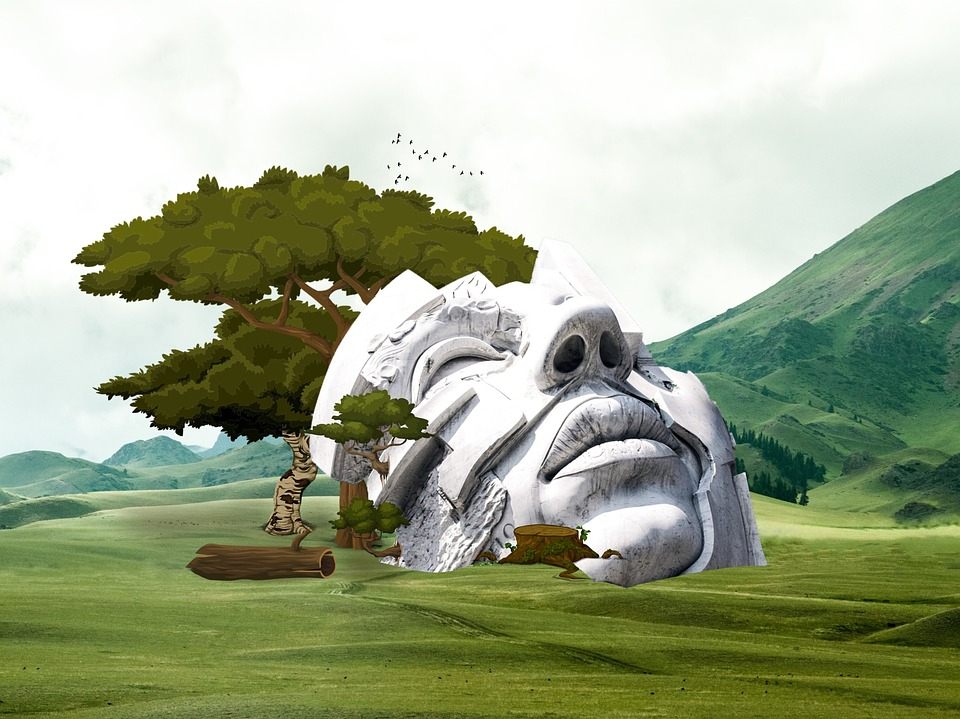
\includegraphics[scale = 0.3]{sbs.jpg}
\caption{Image Side-by-side.}
\label{sbs}
\end{figure}

\subsection{Les flux vidéos en JAVA}

Très peu de bibliothèques manipulant des vidéos existent en JAVA. Au fil des recherches, la première bibliothèque rencontrée est JAVACV\cite{javacv}, qui est un wrapper\footnote{Englobage d'un élément déjà existant
afin de simplifier son utilisation.} autour d'OpenCV. Cependant, les performances de JAVACV sont encore aujourd'hui sujet de débat.\\

Par la suite des bibliothèques multimédia comme Xuggler\cite{xuggler} semblent intéressantes. Xuggler est un wrapper autour de
ffmpeg\footnote{Collection de logiciel libre permettant le traitement de flux audio et vidéos.} pour JAVA. Après quelques essais en ligne de commande de ce qui était offert
par ffmpeg (extraction des frames d'une vidéo, grand nombre de formats décodables,etc...), nous avons voulu tester Xuggler. Malheureusement, cette bibliothèque n'est plus maintenue à jour, en effet le dernier
commit GitHub date de 2014\cite{xugglergit}. En recherchant d'autres wrapper autour de ffmpeg, nous avons opté pour OpenIMAJ\cite{openimaj}.\\

Afin de traiter les flux vidéos et de faire le traitement nécessaire sur les images tirées des vidéos, la bibliothèque OpenImaj parait la plus adaptée car multimédia, et maintenue à jour.
Cette bibliothèque présente de nombreux avantages. Tout d'abord elle est
disponible via un dépot Maven sous forme de modules\cite{openimajmvn}. On peut donc récupérer uniquement les éléments de la bibliothèque
les plus pertinents. Les modules de décodage vidéo et de son sont nécessaires ainsi que ceux de traitements d'images et d'entrées/sorties
Comme dit précédemment, OpenIMAJ est un wrapper ffmpeg. On aura donc l'avantage ici de pouvoir décoder les formats vidéos
les plus utilisés, causant alors très peu de problèmes de compatibilité dans notre
programme.\\

L'encodage quant à lui est par contre beaucoup plus restreint. Cela ne nous empêchera pas de produire
le fichier de sortie dans les formats les plus courants c'est-à-dire MP4, AVI ou MKV.
En ce qui concerne l'image, notre programme donnera en sortie une image au format PNG afin d'éviter la perte de données et
pour pouvoir l'exporter facilement sur le web.

Le son des vidéos sera restitué tel qu'il l'était sur le fichier source.

\section{Cahier des charges et architecture}

\subsection{Cahier des charges}

Besoins fonctionnels :\newline
\begin{itemize}
\item S'affiche sous forme de fenêtre.
\item Choisir le fichier à traiter.
\item Préciser si la vidéo est décodable par le logiciel ou non.
\item Choix du mode de traitement et de l'algorithme (pour l'anaglyphe choisir entre l'algorithme classique ou la méthode
de Dubois).
\item Effectuer le traitement à l'aide d'un bouton.
\item Montrer l'avancement du traitement.
\item Sauvegarder le fichier sous le nom que l'on veut.
\item Pré-visualiser la vidéo sélectionnée\newline
\end{itemize}

Non fonctionnels :\newline
\begin{itemize}
\item Le logiciel doit être rapide. Le traitement doit s'effectuer dans le pire des cas dans le temps de la vidéo.
\item Fidélité. Le logiciel ne doit pas détériorer la qualité de la vidéo originelle.
\newline
\end{itemize}

\subsection{Architecture}

Mon projet sera découpé en différents paquetages, correspondant aux éléments composant le logiciel: traitements, boutons, tests, exceptions et utilitaires (voir figure \ref{arbo}).

\begin{figure}[!h]
\center
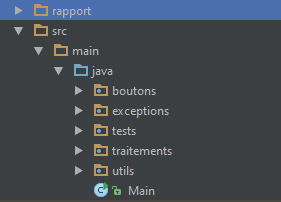
\includegraphics[scale = 1]{tree.PNG}
\caption{Arborescence du projet.}
\label{arbo}
\end{figure}
Le logiciel comprendra une interface simple composée d'un menu permettant de choisir les traitements (voir figure \ref{interface}). En dessous de ce menu se trouveront deux champs permettant de renseigner le fichier vidéo à traiter ainsi que de préciser le fichier de sortie.

\begin{figure}[!h]
\center
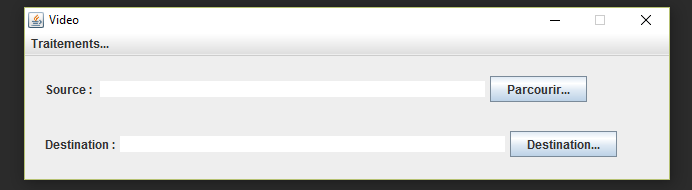
\includegraphics[scale = 0.6]{interface.png}
\caption{Interface principale du logiciel.}
\label{interface}
\end{figure}

Le logiciel comporte deux exceptions. Une de ces exceptions \textit{VideoNonSupporte} est chargée de vérifier si le fichier sélectionné en entrée est supporté par la bibliothèque ou s'il s'agit bien d'une vidéo (voir figure \ref{exception}). OpenImaj ne dispose pas de méthode permettant de vérifier si la vidéo est décodable, l'exception vérifie donc si le fichier sélectionné à un nombre de frames différent de zéro. Une vidéo non décodable ou un fichier quelconque aura un nombre de frame égal à -1 (valeur par défaut dans OpenIMAJ). Lever cette exception interrompt la suite du chargement de la vidéo, elle n'est pas prise en compte.

\begin{figure}[!h]
\center
\includegraphics[scale = 0.7]{exception.PNG}
\caption{Exception lancée par le logiciel.}
\label{exception}
\end{figure}

La deuxième exception se charge de vérifier si un fichier de destination a été précisé. Lors du lancement d'un traitement, si aucun fichier de destination n'est precisé, le traitement ne se lance pas et une boîte de dialogue informe l'utilisateur qu'il faut rentrer un fichier de destination.


Lors de l'appui sur le bouton pour charger une vidéo, c'est la classe ChargerVideo qui est appelée.
Le constructeur de cette classe prend en paramètre un JTextArea et un JPanel. Le JTextArea permet de faire apparaitre le chemin de la vidéo sélectionnée. Le JPanel quant à lui est le conteneur permettant de centrer l'apparition de l'exception \textit{VideoNonSupporte} si le fichier sélectionné ne peut être décodé.\\

Lors de l'appui sur le bouton, un JFileChooser est lancé puis passé à la méthode \textit{chargerVideo(JFileChooser fichier)}.
Cette méthode se charge d'ouvrir la fenêtre de sélection du fichier puis créée 1 flux audio pour la vidéo sélectionnée ainsi qu'un affichage pour visualiser la vidéo. Cette méthode lance l'exception \textit{VideoNonSupporte} si la vidéo n'est pas décodable.
2 flux vidéos sont également créés, l'un servant à être envoyé au traitement et l'autre servant au lecteur vidéo. Il est
nécessaire de charger deux fois la vidéo pour effacer le lien affichage/traitement. En effet, si la vidéo traitée est la même pour l'affichage, regarder la vidéo jusqu'à par exemple la moitié fera commencer le traitement sélectionné à la moitié de la vidéo.

Le bouton permettant de choisir le fichier de destination fait appel à la classe \textit{Sauvegarder} qui elle ne prend en paramètre que le JTextArea pour afficher le chemin du fichier de sortie. Elle fonctionne de manière similaire à la classe de chargement.\\

Une fois ces deux renseignements apportés, l'utilisateur peut alors utiliser le menu des traitements pour choisir lequel appliquer sur sa vidéo (voir figure \ref{menu}). A l'exception du movie barcode, tous les traitements se lancent directement en cliquant sur leur nom (voir figure\ref{menu}). L'utilisateur verra alors un JOptionPane s'afficher, lui indiquant que le traitement est en cours. Tous ces traitements s'exécutent au sein de threads qui permettent à la fenêtre de s'afficher et au traitement de s'exécuter en simultané. Si l'utilisateur choisit par exemple l'anaglyphe, un clic provoque un appel à la classe \textit{ListenerAnaglyphe} qui implémente un \textit{ActionListener}. Cette classe instancie un \textit{ThreadAnaglyphe} et le lance. Cette dernière hérite de \textit{Thread} et lance la méthode \textit{Traitement.anaglyphe()}. 

\begin{figure}[!h]
\center
\includegraphics[scale = 0.6]{menu.png}
\caption{Interface principale du logiciel.}
\label{menu}
\end{figure}

Concernant le movie barcode, un clic sur le menu affiche une fenêtre permettant de saisir les options voulues c'est-à-dire la largeur de l'image et la taille de la bande centrale à récupérer. Ces données sont sauvegardées dans la classe \textit{OptionsBarcode} implémentée en static. Cette fenêtre comporte deux JTextArea, un pour entrer la largeur de l'image et l'autre pour entrer la taille de la bande. Deux clics sur deux boutons \textit{Ok} sont nécessaires pour sauvegarder les valeurs via les méthodes \textit{OptionsBarcode.setLargeur} et \textit{OptionsBarcode.setTailleBande}. Un clic sur le bouton \textit{Valider} permet de lancer le traitement via les threads de manière similaire aux autres traitements.

\begin{figure}[!h]
\center
\includegraphics[scale = 0.6]{barcode.PNG}
\caption{Menu des options pour le movie barcode.}
\label{menu}
\end{figure}

Une fois le traitement sélectionné, un JOptionPane indique que le traitement est en cours via la classe \textit{ThreadEnCours} lancé au début du traitement. Ce JOptionPane est ensuite détruit en fin de traitement et remplacé par un autre indiquant la fin du traitement.

\newpage
\section{Implémentation}

La première chose à réaliser a été de créer le projet Maven\footnote{Outil pour la gestion automatique des projets.}. OpenIMAJ étant disponible via Maven,
Il a été nécessaire de rédiger le fichier pom.xml permettant de récupérer les modules nécessaires. Le fichier est découpé en section à l'aide de balises de façon similaire à l'HTML. Il faut en début de fichier déclarer le projet, sa version, ainsi que les dépôts distants où récupérer les modules.

\lstinputlisting[language=XML, firstline=1, lastline=17,frame=tb,columns=fixed,keywordstyle=\color{blue},breaklines=true,keepspaces,caption = En-tête du ficher pom.xml.]{../pom.xml}

~~\\
Il faut ensuite ouvrir la balise des dépendances et inscrire chaque dépendance que l'on trouve sur le site du dépôt Maven de OpenIMAJ\footnote{https://mvnrepository.com/artifact/org.openimaj}.

\lstinputlisting[language=XML, firstline=19, lastline=32,frame=tb,columns=fixed,keywordstyle=\color{blue},keepspaces,breaklines=true, caption = Dépendances nécessaires.]{../pom.xml}
~~\\

Par la suite, toutes les vidéos résultats seront réalisées grâce à la classe \textit{XuggleVideoWriter} qui permet de créer une vidéo en lui ajoutant chaque frame qui la compose.

\subsection{Movie Barcode}

Le movie barcode doit, pour restaurer la couleur d'une image, récupérer la bande centrale de chaque frame de la vidéo. Il a fallu créer la méthode \textit{getBandeCentrale(MBFImage source)}, qui prend en paramètre une frame et retourne la bande centrale de cette frame. L'algorithme se place au milieu de l'image et la parcourt de $milieu - tailleBande /2$ jusqu'à $milieu + tailleBande /2$ et remplit une nouvelle image de la couleur des pixels de l'image source entre ces bornes. Cette nouvelle image est de hauteur similaire à l'image source et a pour largeur la taille de  la bande. La méthode retourne ensuite cette nouvelle image.

Il faut noter que le  programme ne parcourt que les keyframes de la vidéo, les keyframes étant les seules images codées complètement dans une vidéo, les autres étant calculées à partir des précédentes (P-frame) ou des suivantes (B-frame)\footnote{http://www.dacast.com/blog/what-is-a-key-frame-for-video/}.


L'algorithme parcourt la totalité de la vidéo tant qu'il reste des keyframes ou que la largeur de l'image finale n'a pas été atteinte. Puis, à chaque keyframe rencontrée, sa bande centrale en est extraite et ajoutée à l'image finale à l'aide de la méthode \textit{drawImage (MBFImage imageADessiner, int x, int y)} qui permet de dessiner dans l'objet sur lequel est invoqué la méthode (en l'occurrence ici une image) l'image passée en paramètre aux coordonnées X et Y. Il reste donc suite à l'appel de cette méthode à incrémenter X de la taille de la bande. La boucle while vérifie donc si l'indice de remplissage a atteint la largeur de l'image finale ou qu'il reste des frames dans la vidéo.

\begin{figure}[!h]
\center
\includegraphics[scale = 0.5]{matrix}
\caption{Movie barcode du film \textit{Matrix} généré par le logiciel où la taille de la bande vaut 1 et largeur de l'image vaut 720}
\label{matrix}
\end{figure}

En sortie de cette boucle, l'image est écrite dans le fichier spécifié par l'utilisateur et un JOptionPane l'informe que le traitement est terminé. L'image finale est alors générée (voir figure \ref{matrix}).




\subsection{Side-by-side}
\label{decouper}
Concernant le side-by-side, c'est en étudiant des vidéos produites avec deux sources que j'ai pu me faire une idée de l'algorithme à mettre en œuvre. Outre une perspective différente pour chaque œil, le plus marquant sur une vidéo side-by-side est l'absence ou la présence d'informations sur les bords gauche et droit de l'image. L'image source sera donc tronquée pour reproduire cet effet. L'image perçue par l'œil gauche sera légèrement tronquée sur la droite et l'image perçue par l'œil droit sera légèrement tronquée sur la gauche.
Ce découpage passe par l'appel de deux méthodes \textit{decouperImageGauche()} et \textit{decouperImageDroite()} qui se chargeront de découper les images.

\lstinputlisting[language=JAVA, firstline=364, lastline=370,frame=tb,columns=fixed,keywordstyle=\color{blue},keepspaces, breaklines=true,  basicstyle=\footnotesize, caption = Découpage de l'image gauche.]{../src/main/java/traitements/Traitement.java}
~~\\

La documentation de la méthode \textit{drawImage} nous informe que si l'image de destination est plus petite que l'image source, la copie sera alors tronquée. Il suffit donc pour découper l'image de gauche, de créer une image de destination de taille  (où ESPACEMENT représente le nombre de pixels à tronquer) et de faire appel à la méthode \textit{drawImage} pour obtenir l'image de l'œil gauche qui nous est ensuite retournée.\\

Pour l'image de droite, il n'est pas possible de faire comme précédemment. Il faut alors parcourir l'image source jusqu'à $largeurImageSource - ESPACEMENT$ et copier la couleur des pixels de l'image source dans l'image de destination. Le parcours de la largeur commencera donc à partir de la valeur de la variable \textit{ESPACEMENT}. Il sera alors nécessaire d'avoir un autre indice de remplissage qui lui débutera à 0. Lorsque cet indice aura atteint la largeur de l'image, il faudra alors copier le dernier pixel dans l'image de destination puis remettre la valeur de l'indice à 0. L'image de l'œil droit est ensuite retournée.

Une fois ce découpage effectué il faut alors assembler les deux images ce que fait la méthode \textit{sideBySideImage(MBFImage source)}. Vu que les deux images ont une taille identique qui est $largeurImageSource - ESPACEMENT$, il suffit de créer une image de largeur $(largeurImageSource - ESPACEMENT) * 2$ et de hauteur similaire à l'image source. Par la suite, la méthode \textit{drawImage} est appelée deux fois. Une première fois pour dessiner l'image de l'œil gauche aux coordonnées x = 0 et y = 0, puis une seconde fois pour dessiner l'image de l'œil droit aux coordonnées $x = largeurImageGauche, y = 0$ (voir figure \ref{sbslog}).\\


La méthode \textit{sideBySideImage} est appelée au sein de la méthode \textit{sideByside} qui crée une vidéo de sortie, et ajoute à cette dernière les frames traitées par la méthode \textit{sideBySideImage} via \textit{addFrame(MBFImage frame)}. Cette méthode est fournie par OpenIMAJ et permet l'ajout de n'importe quelle image dans une vidéo. Le format de sortie de la vidéo est quant à lui précisé par l'extension du fichier de sortie que l'utilisateur a saisi plus tôt.

\lstinputlisting[language=JAVA, firstline=247, lastline=271,frame=tb,columns=fixed,keywordstyle=\color{blue},keepspaces, breaklines=true,  basicstyle=\footnotesize, caption = Création de la vidéo.]{../src/main/java/traitements/Traitement.java}


\begin{figure}[!h]
\center
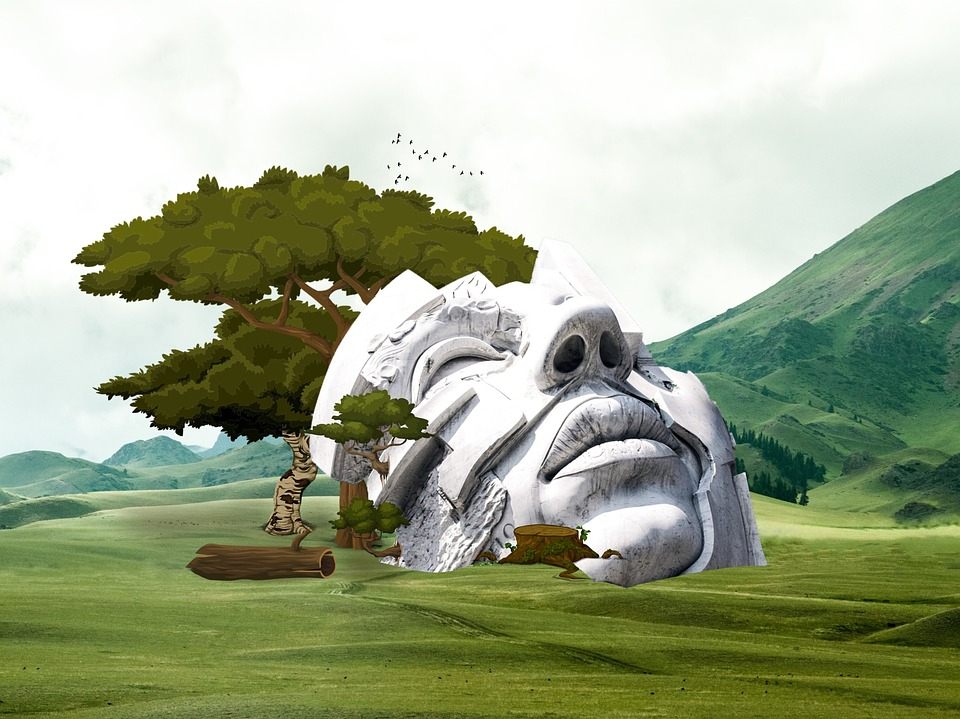
\includegraphics[scale = 0.23]{sbs.png}
\caption{Image side-by-side générée par le logiciel.}
\label{sbslog}
\end{figure}
\newpage
\subsection{Anaglyphe classique et méthode de Dubois}

Pour créer une vidéo possédant l'effet d'anaglyphe, le procédé sera le même que pour le side-by-side. La méthode \textit{anaglyphe()} crée une vidéo de sortie et parcourt l'intégralité des frames de la vidéo source. Les frames anaglyphées sont ensuite ajoutées à la vidéo finale. L'ajout de l'effet d'anaglyphe se fait par la méthode \textit{anaglypheImage(MBFImage source, int largeur, int hauteur)}. 

Cette méthode crée une image de destination en se basant sur la largeur et la hauteur fournit en paramètre et s'occupe de réaliser l'effet anaglyphe en ne traitant pas les bords de l'image. En effet, on ne dispose ici que d'une seule image source. L'algorithme va parcourir l'image en partant d'une valeur de décalage spécifiée dans le code. Pour un point P dans l'image de destination, sa composante rouge sera récupérée en $x - DECALAGE, y$ et sa composante cyan en $x + DECALAGE, y$. Les bords ne peuvent donc pas être traités car le parcours depuis l'origine de l'image provoquerait une sortie des bornes de l'image. Il en est de même pour la fin du parcours de l'image qui se verra arrêér en $largeurImageSource - DECALAGE$ pour éviter un dépassement de bornes. Les composantes rouge et cyan de l'image source sont recopiées dans l'image de destination qui est à la fin du parcours retournée (voir figure \ref{analog}).\\ 

\begin{figure}[!h]
\center
\includegraphics[scale = 0.3]{anaglyphe.png}
\caption{Image anaglyphée générée par le logiciel.}
\label{analog}
\end{figure}  
\newpage
La méthode de Dubois repose sur une matrice pour le changement de la couleur des pixels(voir figure \ref{matrice}). Cette matrice ne peut être utilisée qu'avec deux images. En effet, Éric Dubois ne travaille qu'à partir de deux images prises avec un décalage. L'objectif ici étant de travailler avec une seule image. Il a donc été nécessaire de tronquer l'image source à l'aide  des méthodes \textit{decouperImageGauche} et \textit{decouperImageDroite} comme vu précédemment(voir \ref{decouper}). 

\begin{figure}[!h]
\center
\includegraphics[scale = 0.5]{matrice.png}
\caption{Matrice établie par Éric Dubois.}
\label{matrice}
\end{figure}

Pour un pixel P de l'image source, ses composantes RGB (rouge, vert, bleu) seront soumises à la matrice(voir le résultat figure \ref{anadubois}). Le résultat de ce calcul sera transmis à l'image de destination via la méthode \textit{setPixel}. De manière similaire aux autres algorithmes, une vidéo est créée contenant toutes les frames de la vidéo source, sur lesquelles ont été appliquées la matrice.\\

\begin{figure}[!h]
\center
\includegraphics[scale = 0.3]{anaglyphedubois.png}
\caption{Image anaglyphée selon la méthode de Dubois générée par le logiciel.}
\label{anadubois}
\end{figure}  

\newpage
\section{Phase de test}

Le projet reposant sur la vision stéréoscopique et donc la reconstruction par le cerveau de la perspective, il va être ici compliqué de tester à l'aide d'algorithmes les images obtenues. Cependant, il est possible de tester automatiquement le movie barcode ainsi que le découpage des images qui a lieu lors du side-by-side ou de l'anaglyphe de Dubois.\\ 

L'essentiel de l'algorithme repose sur la récupération de la bande centrale de l'image. Il a fallu implémenter une méthode qui crée une image noire avec une bande centrale rouge. Je fais ensuite appel à la méthode \textit{getBandeCentrale(MBFImage image, int tailleBande)} pour récupérer la bande rouge. Afin de vérifier si le découpage est correct, mon algorithme parcourt la bande et vérifie que tous les pixels sont bien rouges.\\ 

En ce qui concerne le découpage des images, je dispose de deux méthodes créant des images spécifiques pour les tests. Sur une même vue observée par l'œil humain, l'image perçue par l'œil gauche est tronquée sur la droite et inversement pour l'œil droit. La méthode \textit{creationImgGauche()} crée donc une image noire avec une bande rouge sur la droite. La méthode \textit{creationImgDroite()} crée quant à elle une image avec une bande rouge sur la gauche. Le principe ici est donc de vérifier que les deux images ne présentent plus la bande rouge à leurs extrémités après appel à la méthode \textit{Traitement.decouperImageDroite(MBFImage image, int espacement)} et \textit{Traitement.decouperImageGauche(MBFImage image, int espacement)}.

La méthode \textit{testDecouperDroite()} crée l'image de droite et la découpe. Une boucle parcourt ensuite cette dernière afin de vérifier que chaque pixel est bien noir. Il en est de même pour la méthode \textit{testDecouperGauche()}.\\

En ce qui concerne l'anaglyphe classique ou la méthode de Dubois, la seule vérification possible est d'observer le résultat avec des lunettes rouge/cyan (voir figure \ref{analog}). Il n'est pas possible de tester automatiquement la présence ou l'absence de perspective. Observer la reconstruction de l'image complète sur une image de type side-by-side ne peut se faire également qu'avec le matériel adéquat (casque de réalité virtuel pour smartphones\footnote{http://www.homido.com/fr/shop/produits/homido-hmd}, ou appareil plus évolué de type Oculus Rift\footnote{https://www3.oculus.com/en-us/rift/} directement relié à un PC). Il est juste possible d'observer à l'œil deux images légèrement décalées(voir figure \ref{sbslog}).

\newpage
\section{Conclusion}

L'échéance arrivée, le programme remplit ses fonctions. Il est capable d'ouvrir une vidéo et d'effectuer le résumé vidéo, l'anaglyphe classique et selon la méthode de Dubois ainsi que le side-by-side. Le programme prévient l'utilisateur si la vidéo est décodable ou non et si l'utilisateur tente des opérations sans fichier source ou sans fichier de destination.

Des bugs sont néanmoins présents dans le logiciel :\\
\begin{itemize}

\item Lors de la sélection de la vidéo source par l'utilisateur, si le fichier ne présente pas de flux sonore (seulement un flux vidéo), le logiciel n'est pas capable de l'ouvrir. Si aucun flux audio n'est présent, le logiciel n'ouvre pas le fichier.
\item Si l'utilisateur souhaite réaliser deux traitements à la suite nécessitant l'écriture d'une vidéo (side-by-side et anaglyphe par exemple), le premier traitement s'exécutera sans problème, mais le second traitement refusera de se lancer. Le logiciel lancera une erreur d'écriture, affichera une fenêtre indiquant que le traitement est en cours mais ce ne sera pas la cas. En revanche, si l'utilisateur souhaite exécuter un movie barcode à la suite d'un traitement nécessitant l'écriture d'une vidéo, le movie barcode fonctionnera sans problème. On peut donc supposer que la classe \textit{XuggleVideoWriter} est la source du problème.
\item Le programme affiche systématiquement après écriture d'une vidéo une erreur indiquant que l'écriture a échoué. Pourtant le fichier de destination est bien créé.\\

\end{itemize}

Les traitements sont réalisables cependant excepté le résumé vidéo, les autres traitements ne sont pas réalisés en 1/1 (c'est-à-dire dans le temps de la vidéo). En effet les traitements sont deux voire trois fois plus longs que la vidéo. En regardant de plus près le code source d'OpenIMAJ, j'ai pu voir que les pixels sont codés par des flottants entre  0 et 1. Cela pourrait donc induire des temps de calculs plus longs afin de manipuler les nuances de couleurs.

La bibliothèque OpenIMAJ présente également des problèmes de compatibilité entre les différentes plates-formes. Le projet ayant été réalisé majoritairement sous Linux, lors d'un test sur une plate-forme Windows, la bibliothèque est incapable d'ouvrir une vidéo situé sur l'ordinateur. Il en est de même pour les plate-formes MacOS. Il n'est donc utilisable uniquement sous Linux.

La bibliothèque n'est pas capable de restituer du son. En effet, un flux audio peut être ouvert à partir d'une vidéo mais OpenIMAJ ne peut pas le lier à un flux vidéo. Tous les traitements donnent donc pour résultat une vidéo sans son. De plus, lors de l'ouverture de l'audio et de la vidéo lors de la pré-visualisation, les deux se lancent automatiquement. Il est possible de mettre en pause la vidéo mais pas l'audio. L'audio se lance donc sans la vidéo, il est alors nécessaire de lancer la vidéo puis de mettre la lecture sur pause pour que les deux s'arrêtent.

Réaliser deux movie barcode à la suite ne fonctionne pas. En effet, lors du premier movie barcode, la vidéo est parcourue jusqu'à la fin. Donc, lors du lancement du deuxième movie barcode, la vidéo à traiter est déjà à la fin et le movie barcode ne se lance pas. Il faudrait donc implémenter une fonction réinitialisant la position temporelle de la vidéo à 0.

Avec plus de temps, j'aurais pu optimiser mes traitements afin d'atteindre un temps de rendu égal à celui de la vidéo source. J'aurais également pu chercher une bibliothèque gérant mieux le son qu'OpenIMAJ et ne garder OpenIMAJ que pour la gestion de la vidéo et le traitement des images.

\newpage
\bibliography{biblio}


\end{document}